\chapter{Invokedynamic}
\label{chapter:Invokedynamic}
\lhead{ \leftmark }

Though non-Java languages have been running on the JVM since its initial public release, no real effort was made by the engineers within Sun (now Oracle) to make the JVM a hospitable host to languages with semantics that differed from Java.  As more production languages (such as JRuby) used JVM-based runtimes, it became apparent to Sun that more work needed to be done at the JVM level to support these languages.  The goal was to make the JVM more flexible and adaptable while still retaining the strong type verification required to enforce Java's type system.  In order to accomplish this, fundamental changes to the JVM were needed.  These modifications to core JVM functionality, a so-called "renaissance" of the JVM, were created as a branch of the OpenJDK project named the \emph{Da Vinci Machine Project} in mid-2006 and formalized under JSR-292 \cite{jsr-292}.  The finalized implementation was included in the release of JDK 7.  The modifications included low cost function pointers in the form of method handles, new method linking options with the \texttt{invokedynamic} instruction, and changes to the runtime optimizer.

\section{Method Handles}

Before JSR-292, the smallest composable unit within the JVM was the class.  The only available facility to pass invokable references to methods was the Core Reflection API, which was not designed for performance intensive applications.  The Core Reflection API was designed as a meta layer to provide introspection to classes and their declared fields and methods at runtime.  The runtime support for Reflection existed outside of the reach of the JVM optimizer, which meant that reflective invocations could not benefit from optimization heuristics such as inlining \cite{jrose-methodhandles}.  Reflective invocations performed access control checks at each invocation, which resulted in significant overhead at runtime \cite{vmil09}.  Instead of attempting to redefine the behavior of the Core Reflection API and break backwards compatibility, the JSR-292 Expert Group elected to create a new abstraction.  Instead of separate classes to model fields and methods like the existing Core Reflection API, a single interface was created to abstract both field modification and method invocation bytecode instructions: the method handle.

Method handles are function pointers represented as a method descriptor that encapsulate field modification and method invocation operations.  They are represented in the Java standard library in JDK 7 by the \texttt{MethodHandle} class in the \texttt{java.lang.invoke} package.  Unlike the Core Reflection \texttt{Field} and \texttt{Method} classes, a method handle does not exist to provide metadata or perform runtime introspection.  A method handle is meant purely as an efficient means of invoking a functional representation of a bytecode instruction.  Listing \ref{indy-targets-java} defines a class, \texttt{A} with a single field and three methods that are resolved using a \texttt{MethodHandles.Lookup} in Listing \ref{acquire-method-handles}.

\begin{lstlisting}[language=Java,caption=Java field and method lookup targets,label=indy-targets-java]
package test;
class A {
  int value;
  static int a() { ... }
  int b() { ... }
  int c(boolean x) { ... }
}
\end{lstlisting}
\vspace{4em}
\begin{lstlisting}[language=Java,caption=Reflective lookup using \texttt{MethodHandles.Lookup},label=acquire-method-handles]
MethodHandles.Lookup lookup = MethodHandles.lookup();
MethodHandle mh1 = lookup.findGetter(A.class, "value",
                          methodType(int.class));
MethodHandle mh2 = lookup.findStatic(A.class, "a",
                          methodType(int.class));
MethodHandle mh3 = lookup.findVirtual(A.class, "b",
                          methodType(int.class));
MethodHandle mh4 = lookup.findVirtual(A.class, "c",
                          methodType(int.class, boolean.class));
\end{lstlisting}

The descriptors of the method handles acquired in Listing \ref{acquire-method-handles} are listed in Table \ref{table:acquire-method-handles-descriptors}.

\begin{table}[htbp]
  \centering
  \begin{tabular}{ | l | l | p{5cm} |}
  \hline
  \textbf{Method Handle} & \textbf{Descriptor} \\ \hline
  mh1 & \texttt{(Ltest/A;)I} \\ \hline
  mh2 & \texttt{()I} \\ \hline
  mh3 & \texttt{(Ltest/A;)I} \\ \hline
  mh4 & \texttt{(Ltest/A;Z)I} \\ \hline
  \end{tabular}
  \caption[Method Handle Descriptors]{The descriptors of the method handles acquired in Listing \ref{acquire-method-handles}.}
  \label{table:acquire-method-handles-descriptors}
\end{table}

Each \texttt{MethodHandle} can then be called using its \texttt{invoke(Object...)} method, which performs the underlying field access or method invocation.

\section{Method Handle Combinators}

Now that the previously disjoint operations are unified with a common functional abstraction, they can be combined into composite operations.  The potential of method handles is to generate and reconfigure code at runtime without generating and loading raw bytecode into a class loader.  Instead, method handles can be composed with one another -- a function pointer that calls another function pointer -- and integrated with existing class methods to allow flexible code structures constructed solely from method handles that the native code optimizer within the JVM is aware of and able to optimize.

Every bytecode instruction involving data endpoints is representable as a method handle.  These baseline method handles are provided by the \texttt{MethodHandles} class included in the \texttt{java.lang.invoke} package in JDK 7.  The \texttt{MethodHandles} class provides method handles that filter arguments and return values, spread and collect vararg arguments, and conditionally branch between method handles.

\subsection{Filters}
\label{section:filters}

The \texttt{filterArguments()} and \texttt{filterReturnValue()} in the \texttt{MethodHandles} class enable method handles to be adapted to call site descriptors or linked together.  For example, given the classes \texttt{A}, \texttt{B}, and \texttt{C} in Listing \ref{pointer-classes}, evaluating the expression \texttt{a.b.c.value} would require the bytecode listed in Listing \ref{nested-get-bytecode}.

\begin{lstlisting}[language=Java,caption=Classes to execute \texttt{getfield} instructions against,label=pointer-classes]
  class A {
    B b;
  }
  class B {
    C c;
  }
  class C {
    int value;
  }
\end{lstlisting}
\vspace{2em}
\begin{lstlisting}[language=jvm-bytecode,caption=Nested property accessor bytecode,label=nested-get-bytecode]
  aload [a]
  getfield A.b
  getfield B.c
  getfield C.value
\end{lstlisting}

This behavior can now be encapsulated into a single method handle by composing multiple method handles and filtering their return values.  Table \ref{table:method-handle-descriptor-equations} lists equations that describe each method handle performing getfield operations for \texttt{a.b.c.value}.

\begin{table}[htbp]
  \centering
  \begin{tabular}{ | l | l | p{5cm} |}
  \hline
  \textbf{Bytecode Operation} & \textbf{Equation} \\ \hline
  \texttt{getfield A.b} & ${m^{d}}_0 = (A) \to B$ \\ \hline
  \texttt{getfield B.c} & ${m^{d}}_1 = (B) \to C$ \\ \hline
  \texttt{getfield C.value} & ${m^{d}}_2 = (C) \to I$ \\ \hline
  \end{tabular}
  \caption[\texttt{getfield} Descriptors]{Equation representation of the method handle descriptors.}
  \label{table:method-handle-descriptor-equations}
\end{table}

The return value of each method handle is then filtered through the next method handle in the chain:
\[ {m^{d}}_0(A) \to {m^{d}}_1(B) \qquad
   {m^{d}}_1(B) \to {m^{d}}_2(C) \qquad
   {m^{d}}_2(C) \to I \]
After substitution, the method handle tree simplifies down to a method handle that takes an argument of type \texttt{A} and returns the \texttt{int} value of the \texttt{value} field in class \texttt{C}: $\quad{m^{d}}_0(A) \to I  $.

A visual representation of this filtering process is depicted in Figure \ref{fig:pointer-getfield}.

\smallskip
\begin{figure}[htbp]
  \centering
    \includegraphics{./Figures/pointer-getfield.pdf}
  \caption[Method Handle Composition]{A tree of method handles simplify through substitution.}
	\label{fig:pointer-getfield}
\end{figure}

Filtering allows one complex operation to be wrapped into one method handle that can then be invoked, passed as a single object reference to other code, or composed with other method handles for even more complex behavior.

\subsection{Spreaders and Collectors}

A method handle with the descriptor \texttt{(A,B,C)D} could be adapted to a more general method handle with the descriptor \texttt{(Object[])Object} using the \texttt{asVarArgsCollector(Object[].class)} method of the \texttt{MethodHandle} class.  This collects the arguments \texttt{A}, \texttt{B}, and \texttt{C} into the \texttt{Object[]} argument of the adapted method handle.  The inverse operation can be performed with the \texttt{asSpreader(Class<?>, int)} method of the \texttt{MethodHandle} class, which takes all arguments from the provided integer offset and "spreads" them -- distributes them as individual parameters -- back to the original \texttt{(A,B,C)D} form.

\subsection{Guards}

Guards enable the composition of a traditional if-then-else statement using method handles.  Constructing a guard is done by the \texttt{guardWithTest} method within the \texttt{MethodHandles} class which requires three method handles as arguments.  First, a guard predicate which returns a \texttt{boolean} type.  Second, a target method handle to invoke if the guard predicate is true.  Third, a fallback method handle to invoke if the guard predicate is false.  Using another guard as the fallback method handle enables the construction of a tree of conditional branches.

\section{Invocation Linking}

The inflexibility of the JVM prior to JDK 7 stems from the rigidity of the invocation instructions.  The modifications implemented in the Da Vinci Machine Project that make this linkage process more flexible come in the form of a new invocation instruction, \texttt{invokedynamic}.

\subsection{\texttt{invokevirtual} Invocation}

As detailed in Chapter \ref{chapter:JVM}, the JVM uses an internal symbolic linking process to link an invocation instruction, a \emph{callsite}, to the target class method.  During this process the type descriptor embedded in the call site is compared to the type descriptor of the target method and an exception is thrown by the JVM if the type descriptors are not compatible.  A depiction of the linking process for the invocation instruction in Listing \ref{java-normal-invoke-bytecode} is shown in Figure \ref{fig:linking-invokevirtual}.
\vspace{2em}
\begin{lstlisting}[language=jvm-bytecode,caption=virtual method invocation bytecode,label=java-normal-invoke-bytecode]
invokevirtual path/to/OtherClass.otherMethod (I)V
\end{lstlisting}
\vspace{2em}
\begin{figure}[htbp]
	\centering
		\includegraphics[width=\textwidth]{./Figures/linking-invokevirtual.pdf}
	\caption[invokevirtual Linking]{JVM runtime internally resolves symbolic link.}
	\label{fig:linking-invokevirtual}
\end{figure}

\subsection{\texttt{invokedynamic} Invocation}

Instead of a hardwired symbolic link to the target method, \texttt{invokedynamic} call sites embed a symbolic link to a static \emph{bootstrap} method which returns a \texttt{CallSite} object.  The \texttt{CallSite} object contains a \texttt{MethodHandle} which points to the invocation target method.  Simply put, instead of specifying a target method, an \texttt{invokedynamic} call site specifies "who to ask" to get a target method.  Along with the bootstrap method symbolic link, \texttt{invokedynamic} call sites also embed the target method name and type descriptor, which acts as a contract that must be fulfilled by the method handle in the call site returned by the bootstrap method.  An example \texttt{invokedynamic} instruction and corresponding linkage visualization are depicted in Listing \ref{java-indy-invoke-bytecode} and Figure \ref{fig:linking-invokedynamic}, respectively.
\vspace{2em}
\begin{figure}[htbp]
	\centering
    \includegraphics[width=\textwidth]{./Figures/linking-indy-bootstrap.pdf}
	\caption[invokedynamic Linking]{JVM runtime defers to user code bootstrap to resolve symbolic link.}
  \label{fig:linking-invokedynamic}
\end{figure}
\vspace{2em}
\begin{lstlisting}[language=jvm-bytecode,caption=dynamic invocation bytecode,label=java-indy-invoke-bytecode]
invokedynamic
  otherMethod(OtherClass,I)V           // signature being invoked
  path/to/LanguageRuntime.bootstrap    // CallSite provider
  (Lookup, String, MethodType)CallSite // bootstrap signature
\end{lstlisting}

The bootstrap method uses the reflective \texttt{MethodHandle.Lookup} class to obtain method handles, and can optionally perform any combination of method handle adaptation as discussed in Section \ref{section:filters}.  The bootstrap method is defined in JVM bytecode just like any other class, as opposed to the internal JVM process that links the other invocation instructions.  Listing \ref{indy-bootstrap-example} defines an example bootstrap method.

\begin{lstlisting}[language=Java,caption=A bootstrap method,label=indy-bootstrap-example]
class LanguageRuntime {
  static CallSite bootstrap( Lookup lookup,
                             String methodName,
                             MethodType type ) {
    MethodHandle mh = // resolve a MethodHandle ...
    return new MutableCallSite(mh);
  }
}
\end{lstlisting}

\subsection{Call Site Relinking}

\texttt{CallSite} is an abstract base class extended by \texttt{ConstantCallSite} and \texttt{MutableCallSite}.  A \texttt{ConstantCallSite} cannot be re-targeted to another method handle, while the \texttt{MutableCallSite} can be updated with its \texttt{setTarget(MethodHandle)} method.  A \texttt{ConstantCallSite} generally has better performance at the price of flexibility, but the \texttt{MutableCallSite} is useful in building adaptive call sites that are able to rebuild themselves in response to the receivers invoked on them.

\subsection{Optimization}

The primary feature that sets method handles and the \texttt{invokedynamic} infrastructure apart from other JVM features like the Core Reflection API is that method handles are designed to be able to take advantage of many of the optimizations applied to normal bytecode \cite{direct-method-handles}.  Specifically, method handles can be inlined and constant folded as the method handle tree symbols are evaluated and optimized at runtime.

